%for reference to this section
\section{Einleitung}
\label{section:Einleitung} 1350 Wörter

Eine Web Anwendung ein Programm, welches auf einem Server lauft und durch einen Web-Browser kundenseitig abgerufen wird, so \textcite[1]{mahmoud2017}.

Der Transport von Daten, insbesondere sensibler Daten über das Internet, ist Teil der heutigen Webanwendungen, wie \textcite[1]{kirda2009} in ihrem Beitrag erwähnt. Typischerweise interagieren Webanwendungen mit Backend-Datenbanken, um Daten zu empfangen, die später als dynamisch generierte Ausgabe an den Benutzer analysiert werden, wie \textcite[1]{su2006} sagte.

% TODO: Von hier überarbeiten
Die erste Klasse, das gespeicherte XSS, basiert auf Angriffen des Webservers. Das bedeutet, dass bösartiger Code vom Angreifer injiziert und auf einem Webserver gespeichert wird und beim Zugriff auf die Website ausgeführt wird.
Die zweite Klasse, reflektiertes XSS, ist im Grunde genommen das Äquivalent zu gespeichertem XSS mit dem kleinen Unterschied, dass der Code vom Webserver reflektiert wird. Dies kann z.B. der Fall sein, wenn ein Benutzer dazu manipuliert wird, auf einen Link in einer E-Mail zu klicken. Die dritte Klasse und diejenige, mit der sich diese Arbeit am meisten befassen wird, ist DOM-basiertes XSS.\autocite{kirda2009} 

\textcite[]{Sarmah2018} sagte, dass sich DOM-basierte XXS-Angriffe deutlich von den obigen unterscheiden, da es möglich ist, ein bösartiges Skript mit Hilfe des Interpreters im Browser auszuführen.
Außerdem kann es in der Antwort nicht vermerkt werden. Gemäß \textcite[]{Sarmah2018} kann es entweder durch Strukturierung des Document-Object-Models (DOM) gefunden werden oder z.B. zur Laufzeit, wenn eine Webseite geladen wird. 

Um solche XSS-Angriffe zu erkennen, hatten \textcite[]{Wassermann2008} einen der ersten Ansätze zur Erkennung von serverseitig auftretenden Cross Site Scripting (XSS)-Schwachstellen. Kundenseitig wurde die erste Lösung von \textcite[]{Kirda2009} vorgestellt. Sie entwickelten eine Lösung, die auf persönlichen Web-Firewall-Anwendungen basiert, um Cross-Site-Scripting-Angriffe zu reduzieren. Dieses Werkzeug wird als Noxes bezeichnet. Es gibt noch mehr Erkennungsansätze, aber aufgrund der Länge dieser Arbeit werden einige übersprungen.

% TODO: Bis hier überarbeiten

% Einleitungstext......
% wird nach Vollendung aller anderen Texte geschrieben, sowie Abstract und Kurzzusammenfassung.

Web-Anwendungen sind einerseits ein fester Bestandteil wenn es um online Service geht, anderserseits werden immer mehr Anfälligkeiten in solchen entdeckt und offengelgt. \autocite[1]{kirda2009}


\textcite[4]{flanagan2006} erklärt, dass JavaScript eine interpretierte Programmiersprache mit Objectorientierte Möglichkeiten. Sie wird heutzutage großteils dazu genutzt um die client-seitige Darstellung von Webseiten zu verbessern.
JavaScript lauft seit dem Jahr 1997 unter dem Standard ECMAScript\footnote{\url{https://www.ecma-international.org/publications/standards/Ecma-262.htm}} läuft, ist eine Spezifikation davon. Wenn nun ein Web-Browser mit einem JavaScript Interpreter erweitert ist, ermöglicht dieser die Verteilung von ausführbaren Inhalten mittels script.

Nach \textcite[1]{kirda2009} kann vom Interpreter automatisch ausgeführter JavaScript Code einen möglichen Raum für Angriffe gegen die Benutzerumgebung darstellen. Eine sichere Ausführung von JavaScript Code basiert auf dem Prinzip einer Sandbox\footnote{\url{https://de.wikipedia.org/wiki/Sandbox}}. Diese erlaubt es dem Code nur gewisse Operationen auszuführen und gewährt nur begrenzten Zugriff auf Ressourcen im Web-Browser. Ebenso werden JavaScript Programme von verschiedenen Seiten mit einem Abschottungsmechanismus, der "same origin policy"\footnote{\url{https://de.wikipedia.org/wiki/Same-Origin-Policy}} geschützt. Diese erlaubt es dem Programm nur auf Ressourcen innerhalb seines Ursprungs zuzugreifen.

% FIXME: Bild hier oder erst später?
\begin{figure}[ht]
	\centering
	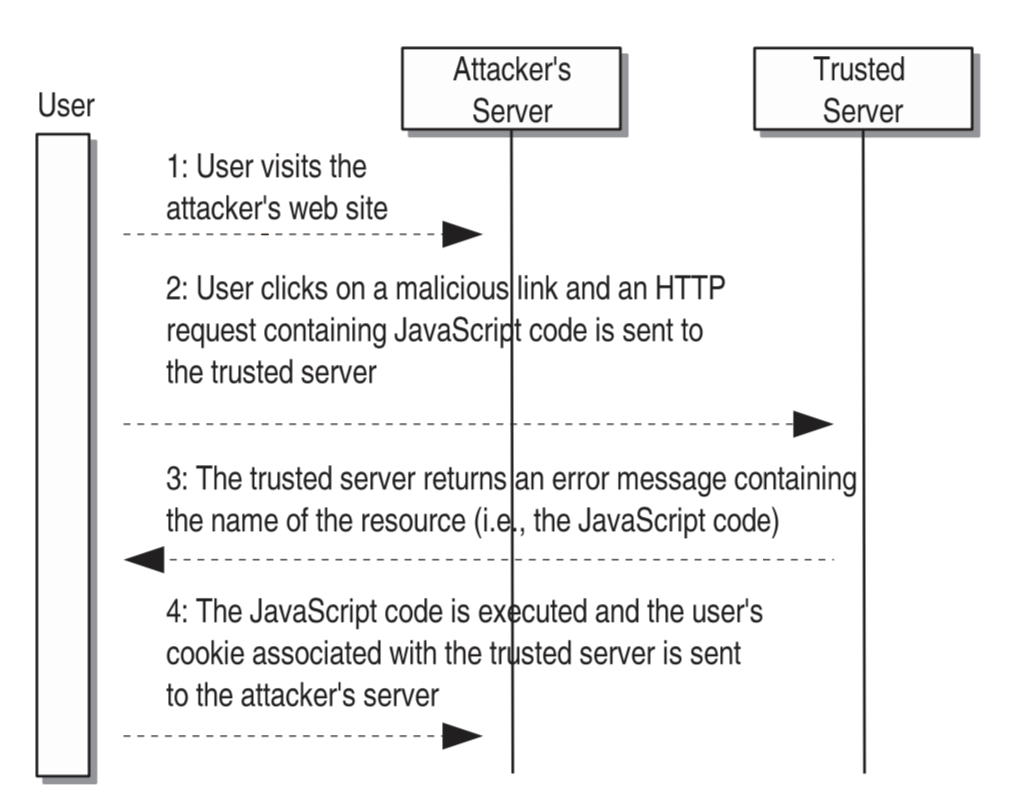
\includegraphics[width=0.5\linewidth]{images/cross-site-scripting_scenario-kirda2009_p2.png}
	\caption{Fig.1 - Ein typischen cross-site scripting Szenarium\autocite[p]{kirda2009}}
\end{figure}

% NEUE Section
\section{Hintergrund und Angriffsarten von XSS}
\label{section:Hintergrund} 1350 Wörter

% genereller Überblick: was ist XXSS und welche Angriffsarten gibt es



In der heutigen Zeit nutzen die meisten Webseiten die Funktionalität von JavaScript im Web-Browser als deren großen Vorteil, doch trotz Einhaltung der "same origin policy" kann immer noch die Sicherheit des Systems verletzt werden. Dies geschieht, wenn beispielsweise ein Nutzer dazu gebracht wird, sich schadhaften JavaScript Code, welcher zuvor von einem Angreifer erstellt worden ist, herunterzuladen. Diese im wahrsten Sinne des Wortes technische Ausbeutung nennt man eine "cross-site scripting"(XSS) Attake.\autocite[2]{kirda2009}


\textcite[2]{hydara2015a} melden, dass diese Sicherheitslücken erstmals in den 1990er, in den frühen Anfängen des World Wide Web, aufgetreten sind. Cross-Site-Scripting(XSS) gehört zu den ernstzunehmendsten Schwächen wenn es um Web Anwendungen geht. Zu Schaden kommen dabei nicht nur der Source Code oder die Datenbank der Web Anwendung, sondern auch der Nutzer.

Laut OWASP \footnote{\url{https://www.owasp.org/index.php/Cross-site_Scripting_(XSS)}} gibt es drei verschiedene Arten, wie XSS Attacken durchgeführt werden können. "reflected", "stored" und "DOM-based". Diese werden grundsätzlich in die zwei Kategorien "reflected" und "stored" unterteilt. Die dritte, viel weniger bekannte Art einer XSS Attacke wird "DOM-based" genannt.

% BUG: 
XSS ist ein Angriff auf den client-seitigen Web-Browser, aber seine Fähigkeiten werden auf der Server-Seite genutzt. Für die Ausnutzung von XSS-Schwachstellen in den Webanwendungen fertigt und injiziert ein Angreifer eine bösartige JavaScript Sprengladung in die Webanwendung. Dieses Skript wird so injiziert, dass es als gutartiger Bestandteil der Website erscheint und schließlich wird dieses Skript in der Domäne des Vertrauens der Website ausgeführt.\autocite[4]{gupta2017}


Beide Arten von XSS Attacken, "reflected" und "stored" werden auf der Server-Seite ausgeführt, und zwar immer dann, wenn eine Anfrage an den infizierten Server geschickt wird. "DOM-based" XSS Attacken werden dahingegen auf der Client-Seite ausgeführt. In allen Fällen sind Angreifer in der Lage sensible Daten von den Opfern zu stehlen.\autocite[2]{hydara2015a}

Der Ablauf um einen solchen Code in die Anwendung injezieren zu können ist immer der Selbe, so \textcite{mahmoud2017}.
\begin{enumerate}
	\item Der Angreifer muss eine Schwachstelle in der Anwendung finden um seinen schadhaften Code in die Anwendung zu bringen und somit in weiterem Verlauf sensible Daten von seinem Opfer stehlen zu können.
	\item Das Opfer besucht die beschädigte Anwendung.
	\item Die Anwendung sendet eine Anfrage mit dem fehlerhaften Code im Body an einen Server.
	\item Wenn das Skript im Web-Browser des Opfers ausgeführt wird, kann der Angreifer diverse persönliche Informationen stehlen.
\end{enumerate}

\begin{figure}[ht]
	\centering
	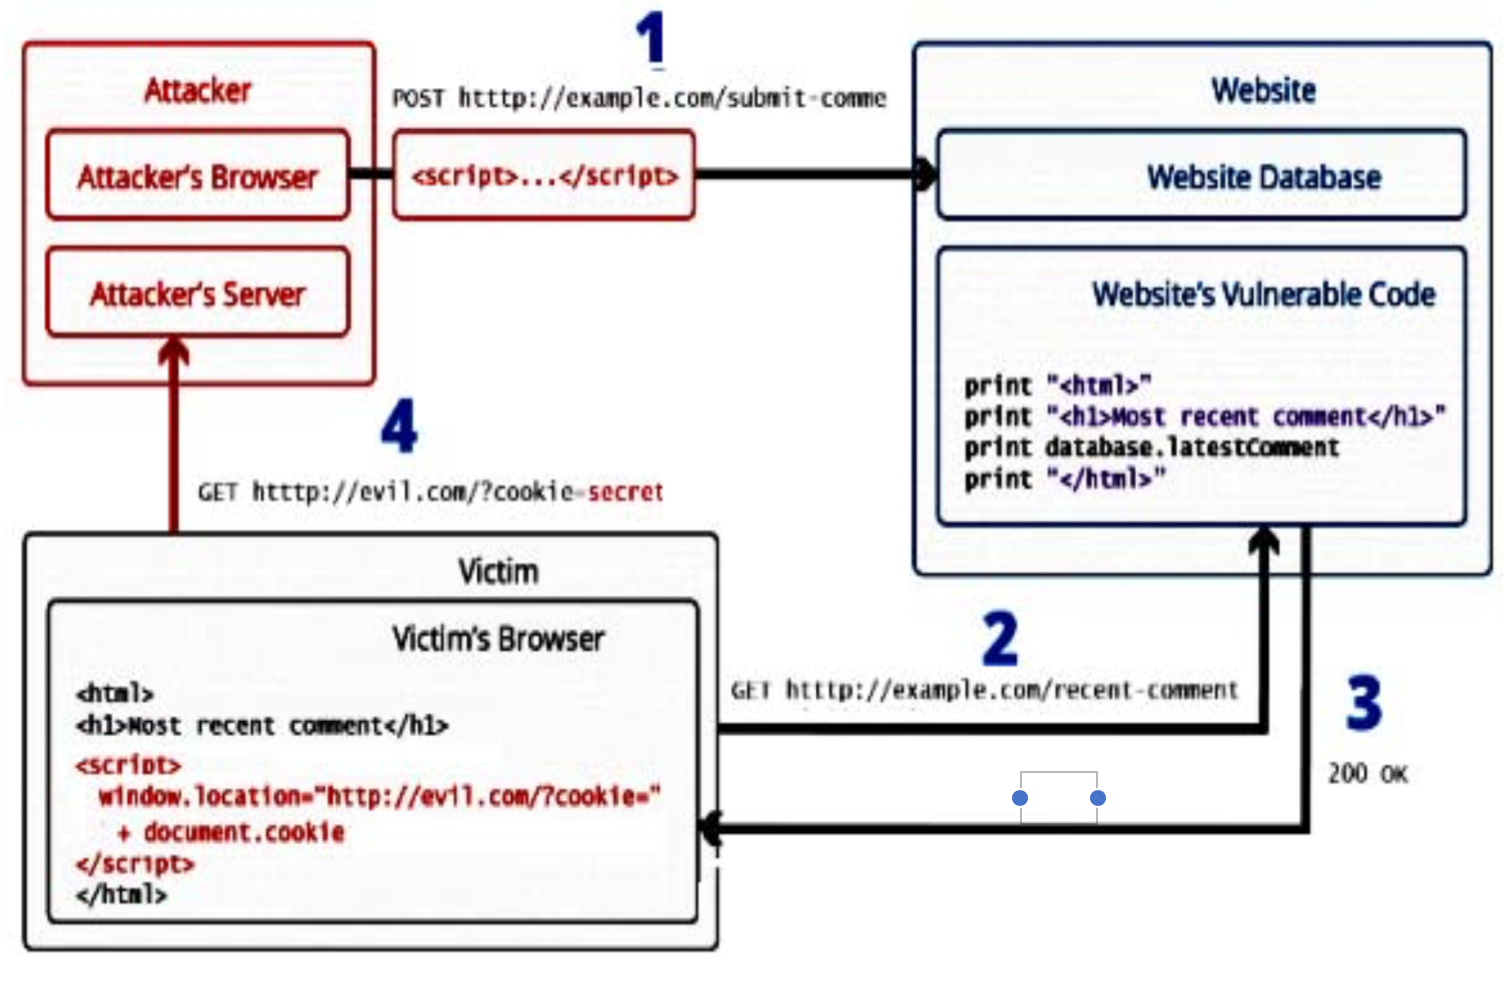
\includegraphics[width=0.75\linewidth]{images/XSS-attack-process.png}
	\caption{XSS Angriffsprozess\autocite[p]{mahmoud2017}}
\end{figure}


% Ab hier genauere Info über Angriffsarten
\subsection{Stored oder Persistent Attacken}
\label{subsection:stored attacks} 350 Wörter

Diese Art von XSS Attacke tritt regelmäßig in sozialen Netzwerken und anderen ähnlichen Web-Anwendungen auf. \textcite[2]{mahmoud2017} nennt diese Schritte um eine Schwachstellen einer XSS Attacke auszunutzen und umzusetzen.
Anders als bei der reflected XSS Attacke wird hierbei der schadhafte Code direkt in die Web-Anwendung oder die Webseite injeziert. Macht der Nutzer nun eine HTTP Anfrage auf den geschädigten Server, so wird der schadhafte Code als Antwort vom Server an das Opfer geschickt und im Web-Browser ausgeführt. Dieses sendet wiederum die Session Cookies des Opfers an die Domain des Angreifers, welcher diese dann dort speichern kann.

\subsection{Reflected oder Non-Persistent Attacken}
\label{subsection:reflective attacks} 350 Wörter

Die Absicht von einer "reflected" XSS Attacke ist es sogenannte Session Cookies \footnote[4]{http://www.allaboutcookies.org/cookies/session-cookies-used-for.html} vom Opfer zu stehlen. Diese Art von XSS Attacke benötigt stärkere Interaktion zwischen Opfer und Angreifer. Folgende Schritte müssen laut \textcite[2]{mahmoud2017} eingehalten werden und diese Attacke erfolgreich durchführen zu können.

Der Angreifer sendet seinem Opfer eine anfangs unscheinbare E-Mail mit einem Link. Dieser Link enthält einen schadhaften JavaScript Code, welcher ausgeführt wird, sobald das Opfer auf diesen klickt. Jetzt wird dieser vorhin platzierte Code an den Server geschickt, ohne dabei von der Web-Anwendung oder der Webseite entdeckt zu werden. In der Antwort des Servers wird dieser Code dem Opfer mitgesandt um somit im weiteren Verlauf die Session Cookies vom Opfer an die Domain des Angreifers zu übermitteln. Der Angreifer kann diese Cookies speichern und in Zukunft immer wieder verwenden.\autocite[2]{mahmoud2017}

\subsection{DOM-basierte Attacken}
\label{subsection:DOM-based Attacks} 350 Wörter

% Die DOM-basierte Attacken



% Neue Section
\section{Erkennunng}
\label{section:Detection} 1350 Wörter

Die Erkennung von Angriffen geht einher mit dessen Ausführung.

\subsection{Methode 1}
\label{subsection:Method1} 675 Wörter

\subsection{Methode 2}
\label{subsection:Method2} 675 Wörter

% Neue Section
\section{Verhinderung} 1350 Wörter
\label{section:Prevention}

\subsection{Methode 1}
\label{subsection:Method1} 675 Wörter

\subsection{Methode 2}
\label{subsection:Method2} 675 Wörter
